\subsection{Throughput percibido en función del delay}

En esta experimentación testeamos el throughput en función del delay de los ACKs.

El objetivo del experimento es ver como impacta el delay en el throughput. Esperamos obtener resultados tales que el delay impacte linealmente, de forma negativa, sobre el throughput

Realizamos mediciones usando distintos tamaños de archivo: 1KB, 5KB, 10KB, 50KB, 100KB y 200KB. Para cada tamaño de archivo medimos el throughput variando el delay en el envío de los ACKs. Los valores de delay que usamos fueron 0.01s, 0.02s, 0.03s, 0.04s, 0.05s, 0.075s, 0.1s.

Por cada tamaño de archivo hicimos 10 corridas, para cada uno de los valores de delay, y promediamos los resultados.

Los valores elegidos para el delay, son en base a pruebas que hicimos haciendo ping a algunos servidores como Google y Facebook, y viendo cuánto es el tiempo que tardan. Los valores obtenidos de RTT obtenidos fueron variados, en promedio de 80ms , así que a partir de eso, fue que decidimos los valores a usar. No aumentamos más de 100ms el delay para las pruebas, ya que al ser muchas pruebas, recopilar la información ya estaba tomando mucho tiempo. 

Aun así hicimos pruebas individuales de tiempos mayores(200 y 500ms) para corroborar que no hubiesen cambios relevantes al aumentar mucho el tiempo de delay, pero vimos que aunque cambiaba en el throughput obtenido, el cambio no era relevante, ya que era similar a variar el delay para valores mas pequeños.

Otra cosa que probamos fue aumentar el delay, más allá del timeout(3 segundos), y vimos que lo que sucedía es que se terminaba perdiendo la conexión. Esto vimos que era porque al superarse el timeout total, el protocolo estimaba que se habían perdido los paquetes y luego de varios intentos se rendía y terminaba la conexión.

A continuación, mostramos los resultados obtenidos para el throughput en función del delay en en un gráfico:


\begin{figure}[H]
	\begin{center}
		  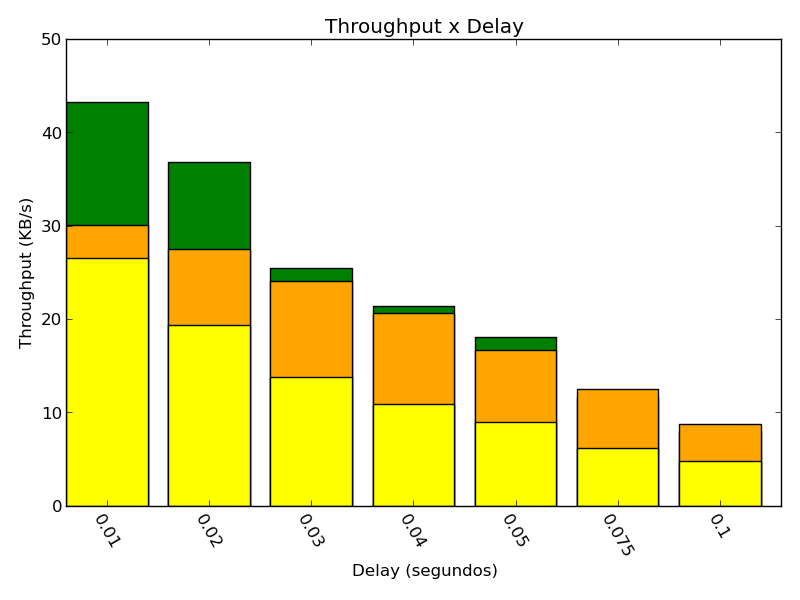
\includegraphics[scale=0.5]{../graficos/test2.png}
		  \caption{$Throughput$ en función del delay para distintos tamaños de archivo}
		  \label{fig:contra1}
	\end{center}
\end{figure}

El gráfico muestra únicamente los resultados para archivos de 1, 10 y 100 KBs. Obviamos incluir los resultados de los otros tamaños, 5, 50 y 200KBs porque resulto que al aumentar el delay, que los throughput medidos resultaban ser muy similares y se encimaban. Eso se puede ver claramente en el gráfico, ya que los throughputs medidos para 1KB y 10KB no se distinguen para delays de 0.075 y 0.1 segundos.

De todas maneras los resultados que se muestran en el gráfico y los demás medidos, nos permiten concluir que efectivamente el throughput disminuye a medida que aumenta el delay. El decremento es casi lineal.
